\chapter{Virtual Memory: Abstraksi, Translasi, Segmentasi, dan Free-Space}
\vspace{1cm}

Virtual memory (VM) adalah salah satu ide paling penting dalam sistem operasi modern. Tanpa VM, programmer harus memikirkan letak fisik data di RAM secara langsung, dan program mudah saling mengganggu. Dengan VM, OS membuat ilusi yang nyaman: setiap proses merasa punya ruang memori sendiri, padahal memori fisik sebenarnya dipakai bersama-sama.

Tujuan utama VM ada tiga:
\begin{itemize}
    \item \textbf{Kemudahan pemrograman:} program melihat ruang alamat yang rapi dan konsisten.
    \item \textbf{Keamanan/proteksi:} proses A tidak bisa sembarang membaca/menulis memori proses B.
    \item \textbf{Efisiensi:} OS bisa menata ulang memori fisik agar pemakaian RAM lebih optimal.
\end{itemize}

Pada bab ini, kita bahas dari konsep dasar sampai praktik pengelolaan ruang bebas. Alurnya sengaja dibuat bertahap: mulai dari "mengapa perlu abstraksi", lalu "bagaimana mesin menerjemahkan alamat", lalu "bagaimana menghemat ruang", sampai "bagaimana allocator mengelola potongan memori yang ukurannya berubah-ubah".

\textbf{Gambaran sederhana untuk siswa SMA:}
anggap RAM seperti apartemen bersama. Banyak siswa (proses) tinggal di satu gedung yang sama (RAM fisik), tetapi tiap siswa merasa punya kamar pribadi (address space virtual). Satpam + manajer gedung (hardware + OS) memastikan tidak ada siswa masuk kamar siswa lain tanpa izin.

\section{Abstraksi Address Space (\textit{vm-intro})}
Pada komputer generasi awal, model memorinya sederhana: OS ada di satu bagian memori fisik, lalu satu program berjalan di sisanya. Ini mudah, tetapi cepat mentok ketika kita ingin menjalankan banyak program sekaligus.

Saat \textit{multiprogramming} dan \textit{time sharing} muncul, kebutuhan berubah drastis. Bayangkan satu komputer dipakai banyak pengguna. Tiap proses harus:
\begin{itemize}
    \item merasa seolah-olah punya memori privat,
    \item tidak boleh merusak proses lain,
    \item tetap bisa dipindah letaknya oleh OS tanpa diketahui program.
\end{itemize}

Di sinilah \textbf{address space} dipakai sebagai abstraksi. Program menulis kode seakan-akan alamat dimulai dari nol dalam ruang miliknya sendiri. Hardware + OS nanti yang menerjemahkan ke alamat fisik sebenarnya.

\textbf{Contoh sederhana:}
dua program berbeda sama-sama menulis ke alamat virtual \texttt{0x1000}. Bagi masing-masing program, alamat itu valid dan "miliknya". Tetapi setelah diterjemahkan, bisa jadi:
\begin{itemize}
    \item Program A $\rightarrow$ alamat fisik 50KB,
    \item Program B $\rightarrow$ alamat fisik 180KB.
\end{itemize}
Jadi alamat virtual sama tidak berarti menabrak di RAM fisik.

\begin{asidebox}{INTI MASALAH: \\ BAGAIMANA MEMVIRTUALISASI MEMORI}
Bagaimana OS memberi ilusi memori privat untuk setiap proses, padahal memori fisik hanya satu dan dipakai bersama?
\end{asidebox}

\begin{figure}[!htbp]
\centering
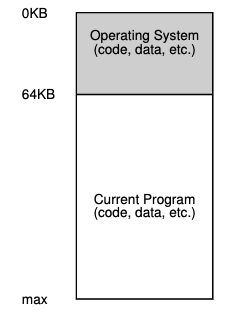
\includegraphics[width=0.55\textwidth,height=0.35\textheight,keepaspectratio]{figures/6_1.png}
\caption{Ilustrasi Sistem Awal: OS dan Satu Program di Memori Fisik}
\label{fig:vmintro-early}
\end{figure}

\textbf{Penjelasan Gambar 6.1 (lebih detail):}
Gambar ini memperlihatkan model paling dasar: memori fisik dibagi untuk OS dan satu program aktif. Keuntungan model ini adalah sederhana dan cepat dipahami. Kekurangannya: tidak skalabel untuk banyak proses. Begitu ada lebih dari satu proses aktif, kita butuh mekanisme tambahan agar pergantian proses tidak mahal dan tidak berbahaya.

\begin{figure}[!htbp]
\centering
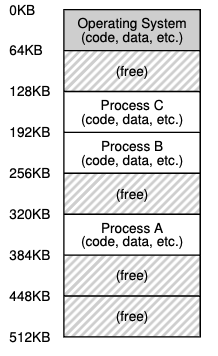
\includegraphics[width=0.28\textwidth,height=0.16\textheight,keepaspectratio]{figures/6_2.png}
\caption{Beberapa Proses Berbagi Memori Fisik}
\label{fig:vmintro-sharing}
\end{figure}

\textbf{Penjelasan Gambar 6.2 (lebih detail):}
Di sini beberapa proses berbagi RAM yang sama. Ini meningkatkan pemanfaatan CPU karena saat proses A menunggu I/O, proses B bisa jalan. Namun risikonya meningkat: kalau tidak ada proteksi, satu bug di proses A dapat menulis ke area proses B. Karena itu konsep isolasi memori menjadi fitur wajib OS modern.

\begin{figure}[!htbp]
\centering
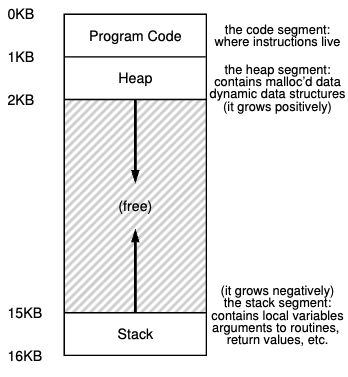
\includegraphics[width=0.52\textwidth,height=0.30\textheight,keepaspectratio]{figures/6_3.png}
\caption{Contoh Struktur Address Space Proses}
\label{fig:vmintro-as}
\end{figure}

\textbf{Penjelasan Gambar 6.3 (lebih detail):}
Address space tipikal berisi:
\begin{itemize}
    \item \textbf{Code/Text:} instruksi program.
    \item \textbf{Data:} variabel global/statis.
    \item \textbf{Heap:} alokasi dinamis (mis. \texttt{malloc}), biasanya tumbuh ke atas.
    \item \textbf{Stack:} frame fungsi lokal, biasanya tumbuh ke bawah.
\end{itemize}
Ruang kosong di antara heap dan stack memberi "ruang napas" agar keduanya bisa tumbuh. Program cukup berpikir dalam ruang virtual ini; OS yang menghubungkan ke RAM nyata.
\textbf{Inti yang perlu diingat:} programmer menulis logika program, bukan mengatur nomor kursi RAM fisik satu per satu.
\FloatBarrier

\section{Interlude API Memori (\textit{vm-api})}
Pada bahasa C, pengelolaan memori berhubungan langsung dengan keandalan program. Kita bisa membagi memori menjadi dua gaya pemakaian:
\begin{itemize}
    \item \textbf{Stack (otomatis):} variabel lokal fungsi; dibuat saat masuk fungsi, hilang saat keluar fungsi.
    \item \textbf{Heap (manual):} dialokasikan saat runtime sesuai kebutuhan; programmer wajib membebaskannya.
\end{itemize}

Dua fungsi kunci:
\begin{itemize}
    \item \texttt{malloc(size)} untuk meminta blok memori,
    \item \texttt{free(ptr)} untuk mengembalikan blok tersebut.
\end{itemize}

Mengapa bagian ini penting? Karena sebagian besar bug memori di C terjadi bukan karena algoritmanya salah, tetapi karena siklus hidup memori tidak disiplin.

\textbf{Bug klasik yang harus dikenali:}
\begin{itemize}
    \item \textit{Memory leak}: memori diminta tetapi tidak pernah dikembalikan.
    \item \textit{Double free}: satu pointer dibebaskan lebih dari sekali.
    \item \textit{Dangling pointer}: pointer masih dipakai padahal memorinya sudah dibebaskan.
    \item \textit{Out-of-bounds write}: menulis melewati ukuran blok, merusak data lain.
\end{itemize}

\textbf{Praktik aman yang disarankan:}
\begin{itemize}
    \item selalu cek hasil \texttt{malloc()} (apakah \texttt{NULL}),
    \item desain jalur \texttt{cleanup} yang jelas untuk kondisi normal dan error,
    \item setelah \texttt{free(ptr)}, set pointer menjadi \texttt{NULL},
    \item cocokkan ukuran alokasi dengan tipe data yang dipakai.
\end{itemize}

Di bawahnya, allocator user-space biasanya meminta ruang besar dari OS (misalnya lewat \texttt{mmap} atau mekanisme lain), lalu memecahnya menjadi blok-blok kecil untuk aplikasi.

\textbf{Ilustrasi alur nyata (ringkas):}
\begin{enumerate}
    \item Program butuh array 1000 elemen.
    \item Program memanggil \texttt{malloc()}.
    \item Allocator mencari blok kosong yang cocok.
    \item Jika tidak ada, allocator meminta ruang baru ke OS.
    \item Alamat blok dikembalikan ke program.
    \item Setelah selesai dipakai, program wajib \texttt{free()}.
\end{enumerate}

\textbf{Checklist aman saat coding C:}
\begin{itemize}
    \item "Siapa yang mengalokasikan, dia juga yang bertanggung jawab membebaskan."
    \item Simpan ukuran buffer dengan jelas.
    \item Hindari menulis dengan indeks yang belum divalidasi.
    \item Uji kasus gagal alokasi, bukan hanya kasus normal.
\end{itemize}

\section{Mekanisme Translasi Alamat (\textit{vm-mechanism})}
Gagasan inti di sini: proses menghasilkan \textit{virtual address}, bukan \textit{physical address}. Hardware kemudian menerjemahkan alamat itu setiap kali terjadi akses memori.

Mekanisme dasar yang paling mudah dipahami adalah \textbf{base-and-bounds}:
\begin{itemize}
    \item \textit{base}: titik awal proses di RAM fisik,
    \item \textit{bounds}: panjang maksimum area legal proses.
\end{itemize}

Alur sederhananya:
\begin{enumerate}
    \item proses mengakses alamat virtual V,
    \item hardware cek apakah V < bounds,
    \item jika valid: physical = base + V,
    \item jika tidak valid: trap ke OS (pelanggaran akses).
\end{enumerate}

Mekanisme ini memberi dua hal sekaligus: cepat (karena sederhana) dan aman (karena ada validasi batas). Meski begitu, model ini punya keterbatasan untuk workload modern yang address space-nya besar dan tidak selalu rapat.

\textbf{Contoh hitung cepat:}
misal \textit{base}=4000 dan \textit{bounds}=1000.
\begin{itemize}
    \item Akses virtual 120 $\rightarrow$ valid, fisik = 4120.
    \item Akses virtual 980 $\rightarrow$ valid, fisik = 4980.
    \item Akses virtual 1200 $\rightarrow$ tidak valid, terjadi trap.
\end{itemize}
Dengan cara ini, proteksi terjadi otomatis pada level hardware.

\begin{figure}[!htbp]
\centering
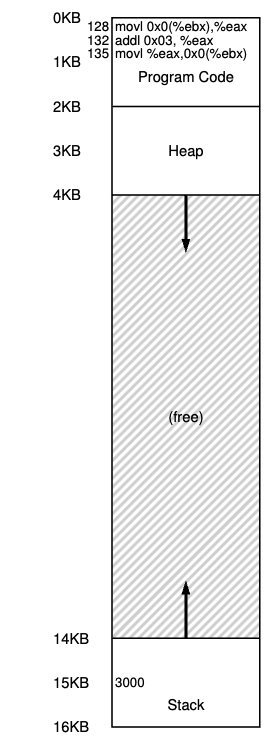
\includegraphics[width=0.52\textwidth,height=0.40\textheight,keepaspectratio]{figures/6_4.png}
\caption{Proses dan Address Space Virtualnya}
\label{fig:vmmech-process}
\end{figure}

\textbf{Penjelasan Gambar 6.4 (lebih detail):}
Program "melihat" peta memori virtual miliknya sendiri. Ini membuat programmer tidak perlu peduli proses lain berada di mana. Efeknya seperti tiap penghuni kos merasa punya alamat kamar sendiri, meskipun sebenarnya bangunannya satu.

\begin{figure}[!htbp]
\centering
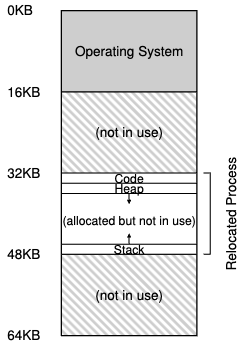
\includegraphics[width=0.48\textwidth,height=0.30\textheight,keepaspectratio]{figures/6_5.png}
\caption{Relokasi Proses di Memori Fisik}
\label{fig:vmmech-relocation}
\end{figure}

\textbf{Penjelasan Gambar 6.5 (lebih detail):}
Relokasi berarti proses dapat dipindah ke lokasi fisik berbeda tanpa mengubah logika program. Ini penting ketika OS melakukan penataan ulang memori, menjalankan banyak proses, atau melakukan context switch.

\begin{figure}[!htbp]
\centering
\scriptsize
\begin{tabular}{|p{0.36\textwidth}|p{0.54\textwidth}|}
\hline
\textbf{Kebutuhan Hardware / Tugas OS} & \textbf{Catatan} \\
\hline
\multicolumn{2}{|l|}{\textbf{A. Kebutuhan Hardware (dynamic relocation)}} \\
\hline
Mode \textit{privileged} & Mencegah proses mode pengguna mengeksekusi operasi khusus kernel. \\
\hline
Register \textit{base} dan \textit{bounds} & Menyimpan titik awal relokasi dan batas legal akses memori proses. \\
\hline
Translasi alamat + cek batas tiap akses & Hardware menerjemahkan alamat virtual dan memvalidasi \textit{out-of-bounds}. \\
\hline
Instruksi \textit{privileged} untuk update base/bounds & Hanya OS yang boleh mengubah nilai translasi sebelum proses dijalankan. \\
\hline
Instruksi \textit{privileged} untuk set handler exception & OS mendaftarkan alamat handler agar trap/exception ditangani benar. \\
\hline
Kemampuan raise exception/trap & Dipicu saat proses mengakses alamat ilegal atau instruksi terlarang. \\
\hline
\multicolumn{2}{|l|}{\textbf{B. Tanggung Jawab OS}} \\
\hline
Saat boot: siapkan trap table/handler & Memastikan exception memori dialihkan ke kernel dengan aman. \\
\hline
Saat membuat proses: alokasikan memori fisik & Menentukan lokasi fisik proses dan ukuran wilayah legalnya. \\
\hline
Saat context switch: muat base/bounds proses aktif & Menjamin translasi selalu sesuai proses yang sedang berjalan. \\
\hline
Saat trap pelanggaran memori: validasi dan tindak lanjut & Menghentikan proses nakal atau memberi sinyal error/proteksi. \\
\hline
Saat proses selesai: bebaskan memori & Mengembalikan ruang fisik ke allocator sistem. \\
\hline
\end{tabular}
\caption{Kebutuhan Hardware dan Tanggung Jawab OS pada Translasi Alamat}
\label{fig:vmmech-hwos}
\end{figure}

\textbf{Penjelasan Gambar 6.6 (lebih detail):}
Tabel ini menegaskan bahwa virtualisasi memori selalu kerja sama dua pihak:
\begin{itemize}
    \item hardware memberi mekanisme cepat dan pemaksaan aturan,
    \item OS mengatur kebijakan dan data kontrolnya.
\end{itemize}
Tanpa hardware, translasi jadi lambat. Tanpa OS, translasi bisa cepat tapi tidak aman atau tidak adil.
\textbf{Kalimat kuncinya:} hardware menjalankan "mesin aturan", OS menentukan "aturan mainnya".
\FloatBarrier

\section{Segmentasi (\textit{vm-segmentation})}
Base-and-bounds tunggal punya kekurangan: ruang kosong besar di address space ikut "terangkut" ke RAM fisik. Segmentasi memecah address space jadi bagian logis agar lebih efisien.

Segmen umum:
\begin{itemize}
    \item code,
    \item heap,
    \item stack.
\end{itemize}

Masing-masing segmen bisa punya base/bounds sendiri. Ini memberi fleksibilitas lebih tinggi daripada satu blok kontigu.

\textbf{Cara baca alamat pada segmentasi (gagasan umum):}
\begin{enumerate}
    \item Ambil beberapa bit atas untuk menentukan nomor segmen.
    \item Sisa bit dipakai sebagai offset dalam segmen itu.
    \item Cek offset terhadap ukuran segmen.
    \item Jika valid, hitung alamat fisik = base segmen + offset.
\end{enumerate}
Proses ini membuat tiap bagian (code/heap/stack) bisa dikelola lebih presisi.

\begin{figure}[!htbp]
\centering
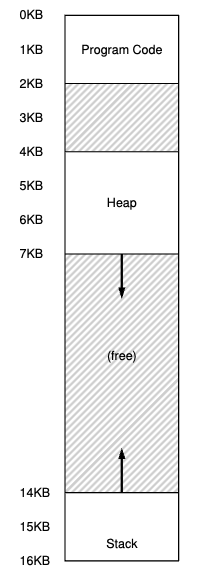
\includegraphics[width=0.48\textwidth,height=0.28\textheight,keepaspectratio]{figures/6_7.png}
\caption{Address Space dengan Celah Ruang Kosong}
\label{fig:vmseg-as}
\end{figure}

\textbf{Penjelasan Gambar 6.7 (lebih detail):}
Celah kosong di antara heap dan stack adalah area yang belum dipakai. Jika kita memaksa memindah address space sebagai satu blok besar, celah ini tetap menghabiskan RAM fisik meskipun tidak membawa data penting.

\begin{figure}[!htbp]
\centering
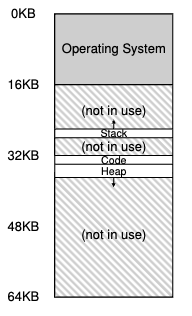
\includegraphics[width=0.52\textwidth,height=0.32\textheight,keepaspectratio]{figures/6_8.png}
\caption{Penempatan Segmen di Memori Fisik}
\label{fig:vmseg-placement}
\end{figure}

\textbf{Penjelasan Gambar 6.8 (lebih detail):}
Dengan segmentasi, code/heap/stack bisa ditempatkan di lokasi fisik berbeda. Hasilnya, ruang RAM bisa diisi lebih rapat dan fleksibel.

\begin{figure}[!htbp]
\centering
\begin{tabular}{|l|c|c|}
\hline
\textbf{Segment} & \textbf{Base} & \textbf{Size} \\
\hline
Code & 32K & 2K \\
\hline
Heap & 34K & 3K \\
\hline
Stack & 28K & 2K \\
\hline
\end{tabular}
\caption{Contoh Nilai Register Segmentasi}
\label{fig:vmseg-registers}
\end{figure}

\textbf{Penjelasan Gambar 6.9 (lebih detail):}
Tiap segmen memiliki parameter sendiri. Artinya, saat translasi berlangsung, sistem perlu tahu alamat virtual itu milik segmen mana dulu, baru memakai base/bounds segmen yang tepat.

\begin{figure}[!htbp]
\centering
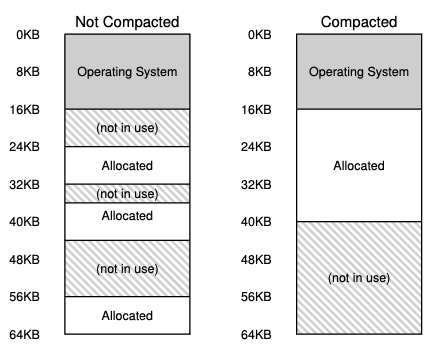
\includegraphics[width=0.56\textwidth,height=0.32\textheight,keepaspectratio]{figures/6_10.png}
\caption{Fragmentasi Eksternal dan Compaction}
\label{fig:vmseg-compaction}
\end{figure}

\textbf{Penjelasan Gambar 6.10 (lebih detail):}
Masalah segmentasi adalah \textbf{fragmentasi eksternal}: ruang kosong banyak tetapi tersebar kecil-kecil. Compaction bisa membantu dengan menggabungkan ruang kosong, tetapi biayanya tinggi karena data harus dipindah.
\textbf{Dampak praktis:}
\begin{itemize}
    \item Sistem jadi perlu waktu ekstra untuk pemindahan data.
    \item Proses aktif dapat terganggu performanya.
    \item Karena mahal, compaction tidak dilakukan sembarangan.
\end{itemize}
\FloatBarrier

\section{Manajemen Free-Space (\textit{vm-freespace})}
Setelah tahu konsep segmentasi, kita masuk ke inti allocator: bagaimana mengelola blok kosong saat ukuran permintaan berubah-ubah.

Analogi sederhana: lemari dengan sekat tidak sama besar. Meski total ruang sisa masih banyak, belum tentu ada satu sekat yang cukup besar untuk barang baru.

Komponen inti allocator:
\begin{itemize}
    \item \textbf{Header}: metadata blok (ukuran/status),
    \item \textbf{Free list}: daftar blok kosong,
    \item \textbf{Split}: pecah blok besar jadi beberapa bagian,
    \item \textbf{Coalesce}: gabung blok kosong yang berdampingan.
\end{itemize}

\textbf{Strategi pemilihan blok (trade-off):}
\begin{itemize}
    \item \textit{First fit}: ambil blok pertama yang cukup; cepat, tapi bisa memicu fragmentasi.
    \item \textit{Best fit}: ambil blok paling pas; hemat sisa kecil, tapi pencarian bisa lebih lama.
    \item \textit{Worst fit}: ambil blok terbesar; kadang menyisakan blok besar berguna, tetapi tidak selalu efisien.
\end{itemize}

\textbf{Ilustrasi singkat:}
jika ada blok kosong 20KB, 8KB, 6KB dan permintaan 5KB:
\begin{itemize}
    \item first fit mungkin mengambil 20KB (sisa 15KB),
    \item best fit akan memilih 6KB (sisa 1KB),
    \item worst fit memilih 20KB (sama seperti first fit di contoh ini).
\end{itemize}
Pilihan strategi mempengaruhi bentuk free list dalam jangka panjang.

\begin{figure}[!htbp]
\centering
\begin{minipage}[t]{0.48\textwidth}
\centering
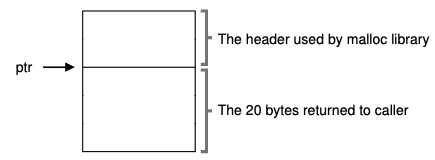
\includegraphics[width=\textwidth,height=0.26\textheight,keepaspectratio]{figures/6_11a.png}\\
\small (a)
\end{minipage}
\hfill
\begin{minipage}[t]{0.48\textwidth}
\centering
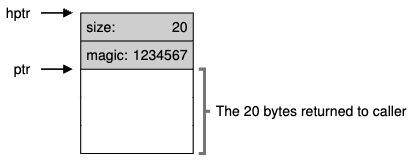
\includegraphics[width=\textwidth,height=0.26\textheight,keepaspectratio]{figures/6_11b.png}\\
\small (b)
\end{minipage}
\caption{Header Blok Alokasi pada Heap}
\label{fig:vmfree-header}
\end{figure}

\textbf{Penjelasan Gambar 6.11(a)-(b) (lebih detail):}
Gambar ini memperlihatkan bahwa allocator bukan hanya menyimpan data user, tapi juga metadata. Metadata inilah yang membantu allocator tahu batas blok, status terpakai/kosong, dan memproses \texttt{free()} dengan benar.

\begin{figure}[!htbp]
\centering
\begin{minipage}[t]{0.48\textwidth}
\centering
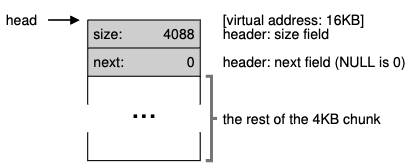
\includegraphics[width=\textwidth,height=0.26\textheight,keepaspectratio]{figures/6_12a.png}\\
\small (a)
\end{minipage}
\hfill
\begin{minipage}[t]{0.48\textwidth}
\centering
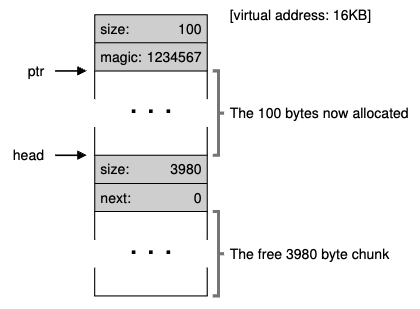
\includegraphics[width=\textwidth,height=0.26\textheight,keepaspectratio]{figures/6_12b.png}\\
\small (b)
\end{minipage}
\caption{Perubahan Heap Saat Alokasi Awal}
\label{fig:vmfree-alloc}
\end{figure}

\textbf{Penjelasan Gambar 6.12(a)-(b) (lebih detail):}
Perubahan ini menunjukkan efek operasi alokasi terhadap struktur heap. Setelah alokasi, bentuk free list berubah. Jika desain allocator buruk, perubahan ini lama-lama menimbulkan fragmentasi berat.

\begin{figure}[!htbp]
\centering
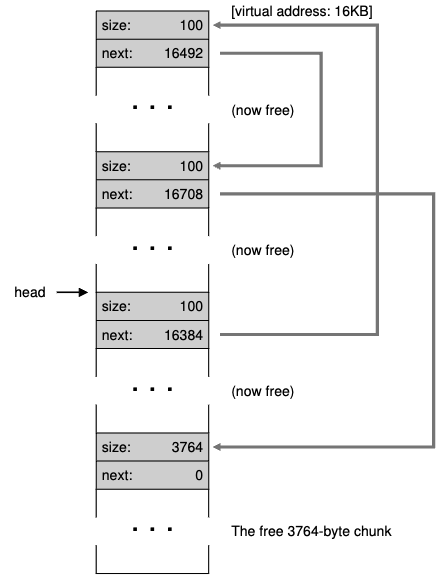
\includegraphics[width=0.56\textwidth,height=0.30\textheight,keepaspectratio]{figures/6_13.png}
\caption{Contoh Free List Tanpa Coalescing}
\label{fig:vmfree-nocoalesce}
\end{figure}

\textbf{Penjelasan Gambar 6.13 (lebih detail):}
Tanpa coalescing, blok kosong kecil tetap terpisah-pisah. Akibatnya, permintaan memori besar dapat gagal meskipun total ruang kosong cukup jika dijumlah.

\begin{figure}[!htbp]
\centering
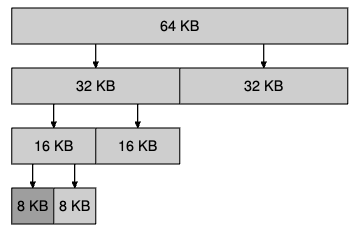
\includegraphics[width=0.56\textwidth,height=0.30\textheight,keepaspectratio]{figures/6_14.png}
\caption{Contoh Buddy System}
\label{fig:vmfree-buddy}
\end{figure}

\textbf{Penjelasan Gambar 6.14 (lebih detail):}
Buddy system memecah blok dengan pola ukuran tertentu (biasanya pangkat dua). Keuntungan utamanya: proses gabung/kembali (merge) blok jadi lebih cepat dan teratur. Kekurangannya: bisa muncul \textit{internal fragmentation} saat ukuran yang diminta tidak pas.
\textbf{Contoh:} program minta 10KB, sistem mungkin memberi 16KB karena ukuran terdekat di buddy level itu. Sisa 6KB di dalam blok tidak terpakai oleh user, tetapi tetap terhitung teralokasi.
\FloatBarrier

\section{Ringkasan Bab}
Ringkasan lengkap bab ini:
\begin{enumerate}
    \item Address space adalah abstraksi yang membuat program tidak perlu tahu posisi fisik data.
    \item Proteksi memori adalah syarat wajib saat banyak proses berbagi RAM.
    \item Translasi virtual-ke-fisik dilakukan sangat sering, sehingga butuh dukungan hardware.
    \item Base-and-bounds adalah model awal yang mudah dipahami dan cukup aman.
    \item Segmentasi meningkatkan efisiensi karena address space tidak diperlakukan satu blok utuh.
    \item Fragmentasi eksternal adalah masalah utama pada alokasi ukuran variabel.
    \item Allocator butuh metadata dan strategi pemilihan blok yang tepat.
    \item Coalescing penting untuk menjaga kualitas free list dalam jangka panjang.
    \item Buddy system menawarkan manajemen yang rapi dengan trade-off tertentu.
    \item Inti desain VM selalu tentang trade-off: sederhana vs fleksibel, cepat vs efisien ruang.
\end{enumerate}

\section*{Referensi}
\begin{itemize}
    \item Arpaci-Dusseau, R. H., dan Arpaci-Dusseau, A. C. \textit{Operating Systems: Three Easy Pieces (OSTEP)}.
    \item Chapter 13: \textit{The Abstraction: Address Spaces}.
    \item Chapter 14: \textit{Interlude: Memory API}.
    \item Chapter 15: \textit{Mechanism: Address Translation}.
    \item Chapter 16: \textit{Segmentation}.
    \item Chapter 17: \textit{Free-Space Management}.
\end{itemize}

\section*{Pekerjaan Rumah (Konseptual)}
\textbf{Pertanyaan}
\begin{enumerate}
    \item Mengapa address space disebut ilusi yang berguna bagi programmer?
    \item Jelaskan dengan contoh bagaimana base-and-bounds melindungi proses.
    \item Bedakan stack vs heap dari sisi umur data dan cara pengelolaannya.
    \item Mengapa segmentasi bisa lebih hemat RAM dibanding satu blok kontigu?
    \item Jelaskan bedanya fragmentasi eksternal dan internal dengan contoh.
    \item Mengapa coalescing penting dalam allocator jangka panjang?
    \item Kapan buddy system lebih baik dipakai daripada free list biasa?
\end{enumerate}
